\chapter{Return on Investment and Operational Profit}
\label{sec:roi}

The return on investment (ROI) analysis evaluates whether the selected BELLONA concept can become financially viable as a commercial product. The analysis uses the updated company-level profit-and-loss and cash-flow model, rather than the simplified baseline estimate, because this model includes unit production cost, development effort, operating expenses, recurring service cost, tax, capital expenditure, and financing needs. 

\section{Financial Model Scope and Key Assumptions}

BELLONA is assumed to follow a direct product-sale business model with additional annual maintenance and service revenue. One unit is defined as one complete deployable unmanned aircraft system (UAS) package, including the aircraft, balloon-interaction mechanism, ground/support equipment, commissioning, and customer handover. An airport-equivalent deployment is assumed to require three units on average, providing coverage of the complete airport flight zone while maintaining operational availability during charging, inspection, or maintenance.

The main financial assumptions used in the model are summarised in Table~\ref{tab:roi_key_assumptions}. Values are based on the BELLONA financial plan.

\begin{center} % longtable centers itself by default, but standard environment wrapping applies
\small
\renewcommand{\arraystretch}{0.95} 
% Total width matches your previous 0.4\textwidth + 0.58\textwidth = 0.98\textwidth
\begin{longtable}{p{0.4\textwidth}p{0.58\textwidth}}
    
    % --- FIRST PAGE HEADER (Caption goes here) ---
    \caption{Key financial assumptions used for the BELLONA ROI model.} \label{tab:roi_key_assumptions} \\
    \toprule
    \textbf{Parameter} & \textbf{Value used in model} \\
    \midrule
    \endfirsthead
    
    % --- SUBSEQUENT PAGES HEADER (No caption) ---
    \toprule
    \textbf{Parameter} & \textbf{Value used in model} \\
    \midrule
    \endhead
    
    % --- FINAL FOOTER ---
    \bottomrule
    \endlastfoot

    % --- DATA ROWS ---
    Business model & Direct product sale + annual maintenance/service revenue \\
    Unit definition & One complete deployable UAS package \\
    Average airport-equivalent deployment & 3 units \\
    Unit sales price & EUR 24,875 per new unit \\
    Annual maintenance/service revenue & EUR 11,999 per active unit / year \\
    One-time Cost of Goods Sold (COGS) & EUR 17,100 per new unit \\
    Recurring COGS & EUR 2,400 per active unit / year \\
    Direct operator mission cost & EUR 150 per mission \\
    Target year & Year 6 \\
    Year 6 active installed base & 159 units \\
    Year 6 revenue & EUR 3.67M \\
    Year 6 net profit & EUR 89k \\
    Total external funding required & EUR 3.15M \\
\end{longtable}
\vspace{-20pt}

\end{center}
\section{Market Volume and Sales Ramp}

The commercial ramp is based on a regional beachhead market, not the full global counter-UAS market. Initial target customers include airports, border-security agencies, national authorities, and selected critical-infrastructure operators in European border regions exposed to balloon-based smuggling or hybrid airspace disruption. Therefore, the market is not treated as airport-only, since the Year 6 installed base would be too aggressive if justified only by airports in a small number of countries.

For the midterm estimate, the serviceable available market is taken as approximately 150--180 airport-equivalent deployment sites. With three BELLONA units per site, this corresponds to approximately 450--540 serviceable units. The Year 6 installed base of 159 units therefore represents an achievable market share of approximately 29--35\% of the initial serviceable market. This is ambitious but defensible for a first-mover product in a narrow threat niche, provided that customers include airports, border authorities, and critical infrastructure operators.

\begin{figure}[H]
    \centering
    \begin{tikzpicture}[
        box/.style={
            rectangle,
            rounded corners=1.5mm,
            draw=black,
            fill=gray!10,
            text width=0.21\textwidth, % Mathematically fits 4 boxes perfectly within 1.0\textwidth
            minimum height=4.2cm,      % Height adjusted slightly upward to handle the narrower wrap
            inner sep=1.2mm,           % Tightened side padding to maximize text space
            align=center,
            font=\footnotesize         % Slightly smaller base font to prevent text clipping/hyphenation
        },
        arrow/.style={
            -{Latex[length=2mm]},
            thick
        },
        node distance=0.25cm % Small, controlled gap to prevent margin overflow
    ]

    \node[box] (sites) {
        \textbf{Regional serviceable deployment sites}\\
        \vspace{1mm}
        150--180 airports, border-security sites, national authority sites, and critical-infrastructure locations
    };

    \node[box, right=of sites] (units) {
        \textbf{Serviceable unit market}\\
        \vspace{1mm}
        450--540 BELLONA units\\
        \vspace{1mm}
        Assuming 3 units per airport-equivalent deployment site
    };

    \node[box, right=of units] (installed) {
        \textbf{Year 6 installed base}\\
        \vspace{1mm}
        159 active BELLONA units\\
        \vspace{1mm}
        Equivalent to approximately 53 airport-equivalent deployments
    };

    \node[box, right=of installed] (share) {
        \textbf{Implied Year 6 market share}\\
        \vspace{1mm}
        29--35\% of the initial regional serviceable unit market
    };

    \draw[arrow] (sites) -- (units);
    \draw[arrow] (units) -- (installed);
    \draw[arrow] (installed) -- (share);

    \end{tikzpicture}
    \caption{Market interpretation of the Year 6 installed base.}
    \label{fig:roi_market_funnel}
\end{figure}
Commercial entry starts in Year 2 with the first five units sold, followed by a gradual increase in annual deliveries as customer adoption, production capacity, and service capability grow. The installed base reaches 159 active units by Year 6, equivalent to approximately 53 airport-equivalent deployments. This installed base is the main driver of long-term financial viability because recurring maintenance and service revenue scales with active units rather than only with new sales.
\begin{figure}[H]
    \centering

    \begin{subfigure}[b]{0.48\textwidth}
        \centering
        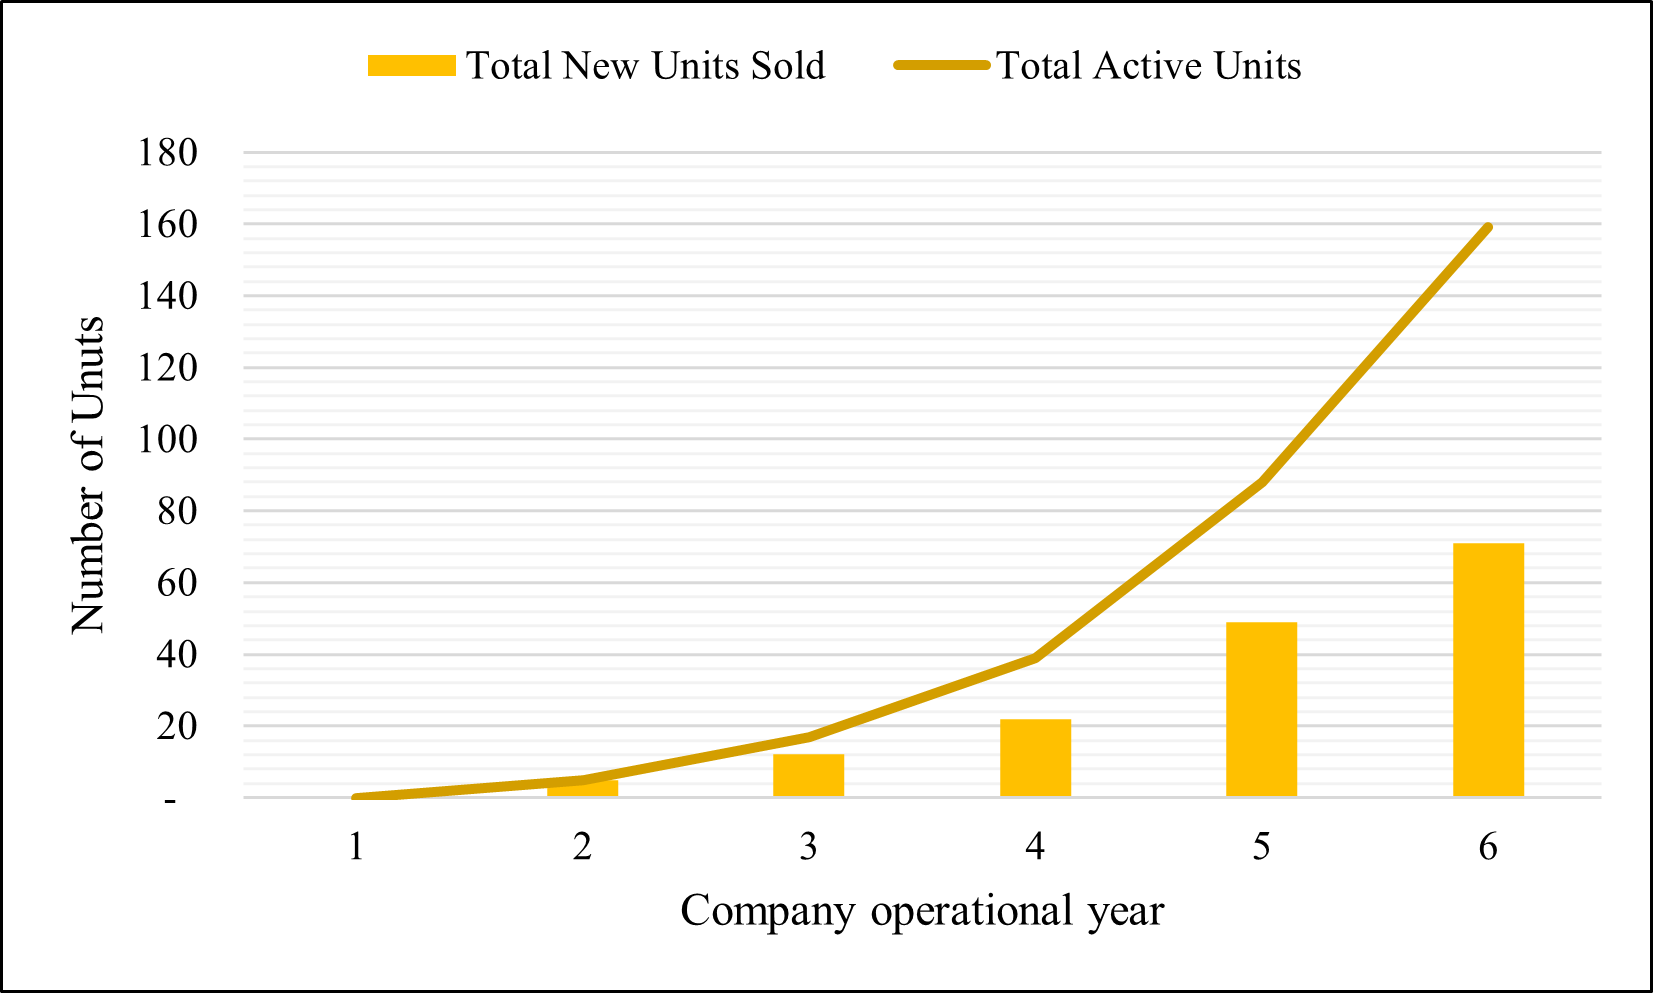
\includegraphics[width=\textwidth]{figures/Chart Number of Units.png}
        \caption{Projected sales ramp and active installed base.}
        \label{fig:roi_sales_ramp}
    \end{subfigure}
    \hfill
    \begin{subfigure}[b]{0.48\textwidth}
        \centering
        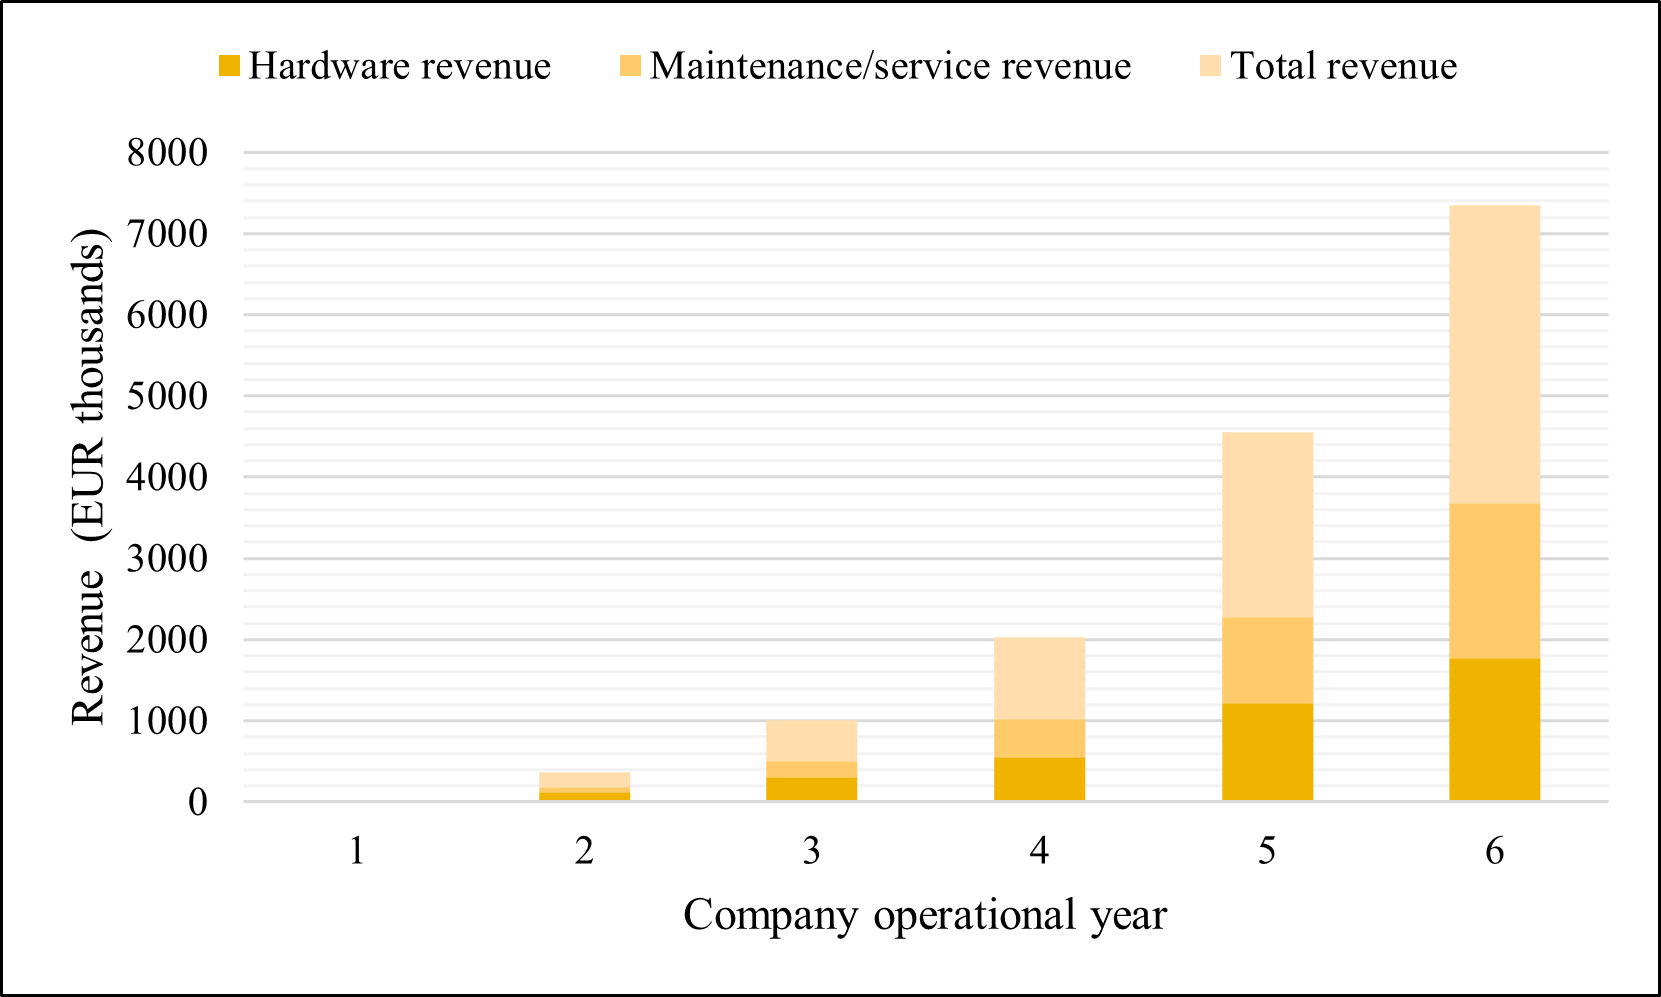
\includegraphics[width=\textwidth]{figures/Chart revenue.png}
        \caption{Revenue split (New units vs. Recurring service).}
        \label{fig:roi_revenue_split}
    \end{subfigure}

    \caption{Sales and revenue projections for BELLONA from Year 1 to Year 6.}
    \label{fig:roi_sales_revenue}
\end{figure}

\begin{figure}[H]
    \centering

    \begin{subfigure}[b]{0.48\textwidth}
        \centering
        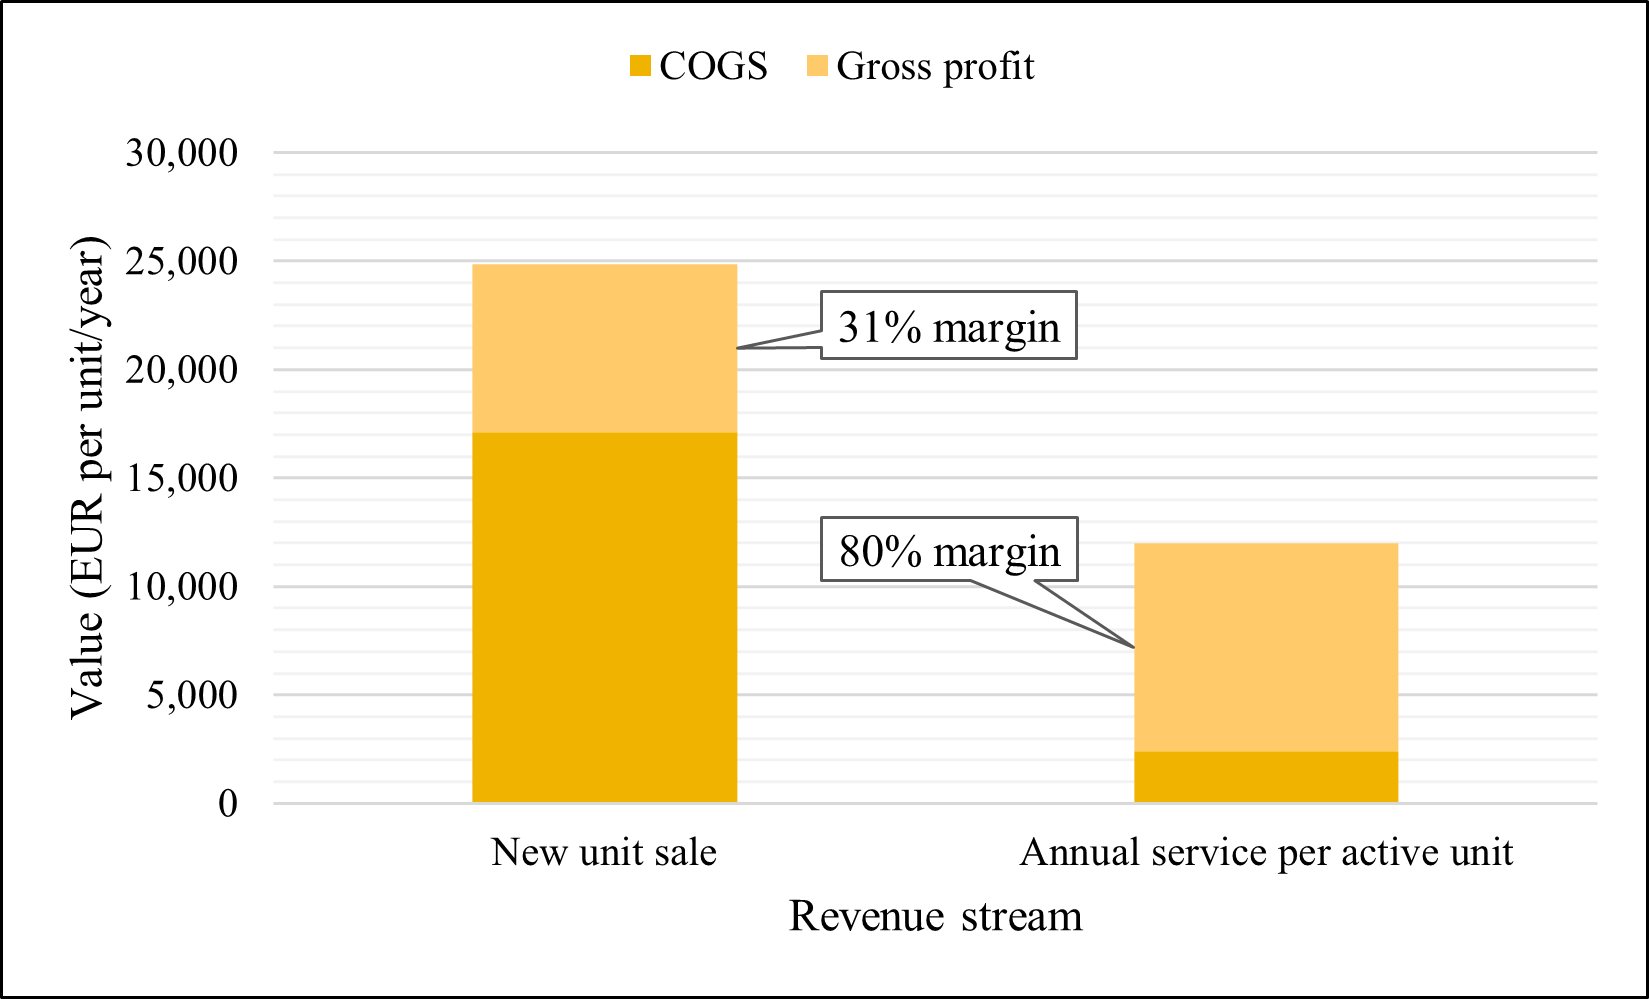
\includegraphics[width=\textwidth]{figures/Chart Profits.png}
        \caption{Unit-level gross margins.}
        \label{fig:roi_unit_economics}
    \end{subfigure}
    \hfill
    \begin{subfigure}[b]{0.48\textwidth}
        \centering
        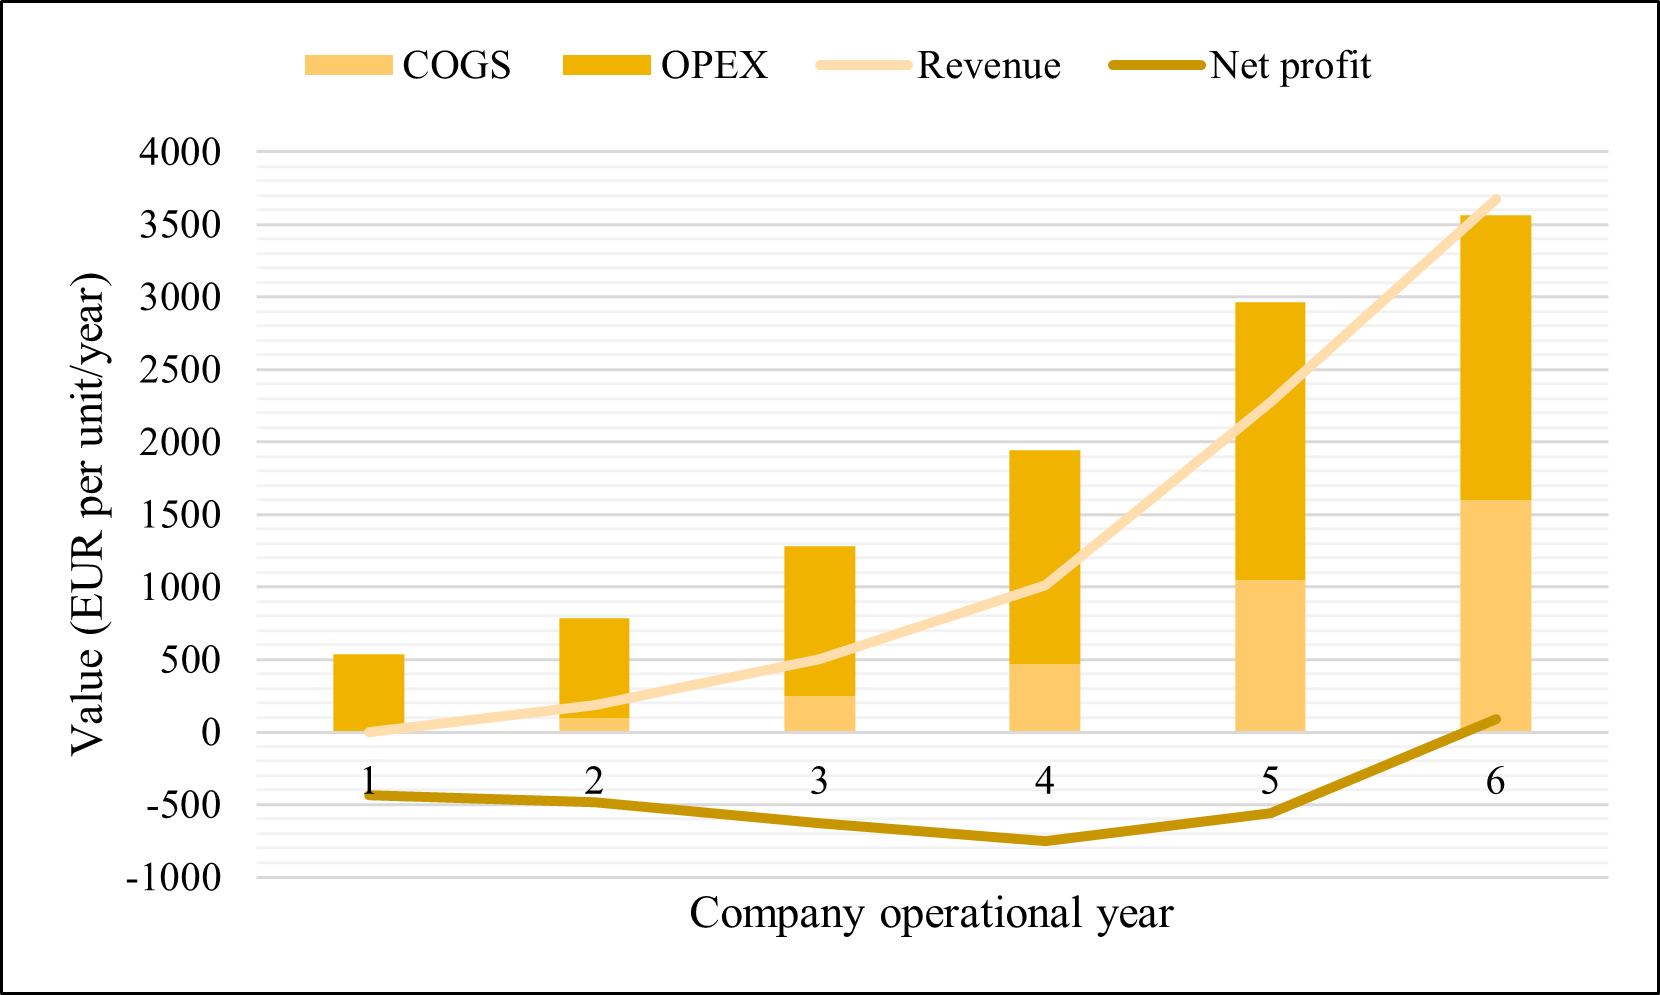
\includegraphics[width=\textwidth]{figures/Chart P&L.png}
        \caption{Profit-and-loss development.}
        \label{fig:roi_pl_development}
    \end{subfigure}

    \caption{Margin and profit-and-loss projections for BELLONA from Year 1 to Year 6.}
    \label{fig:roi_profit_overview}
\end{figure}
%\begin{figure}[H]
 %   \centering
 %   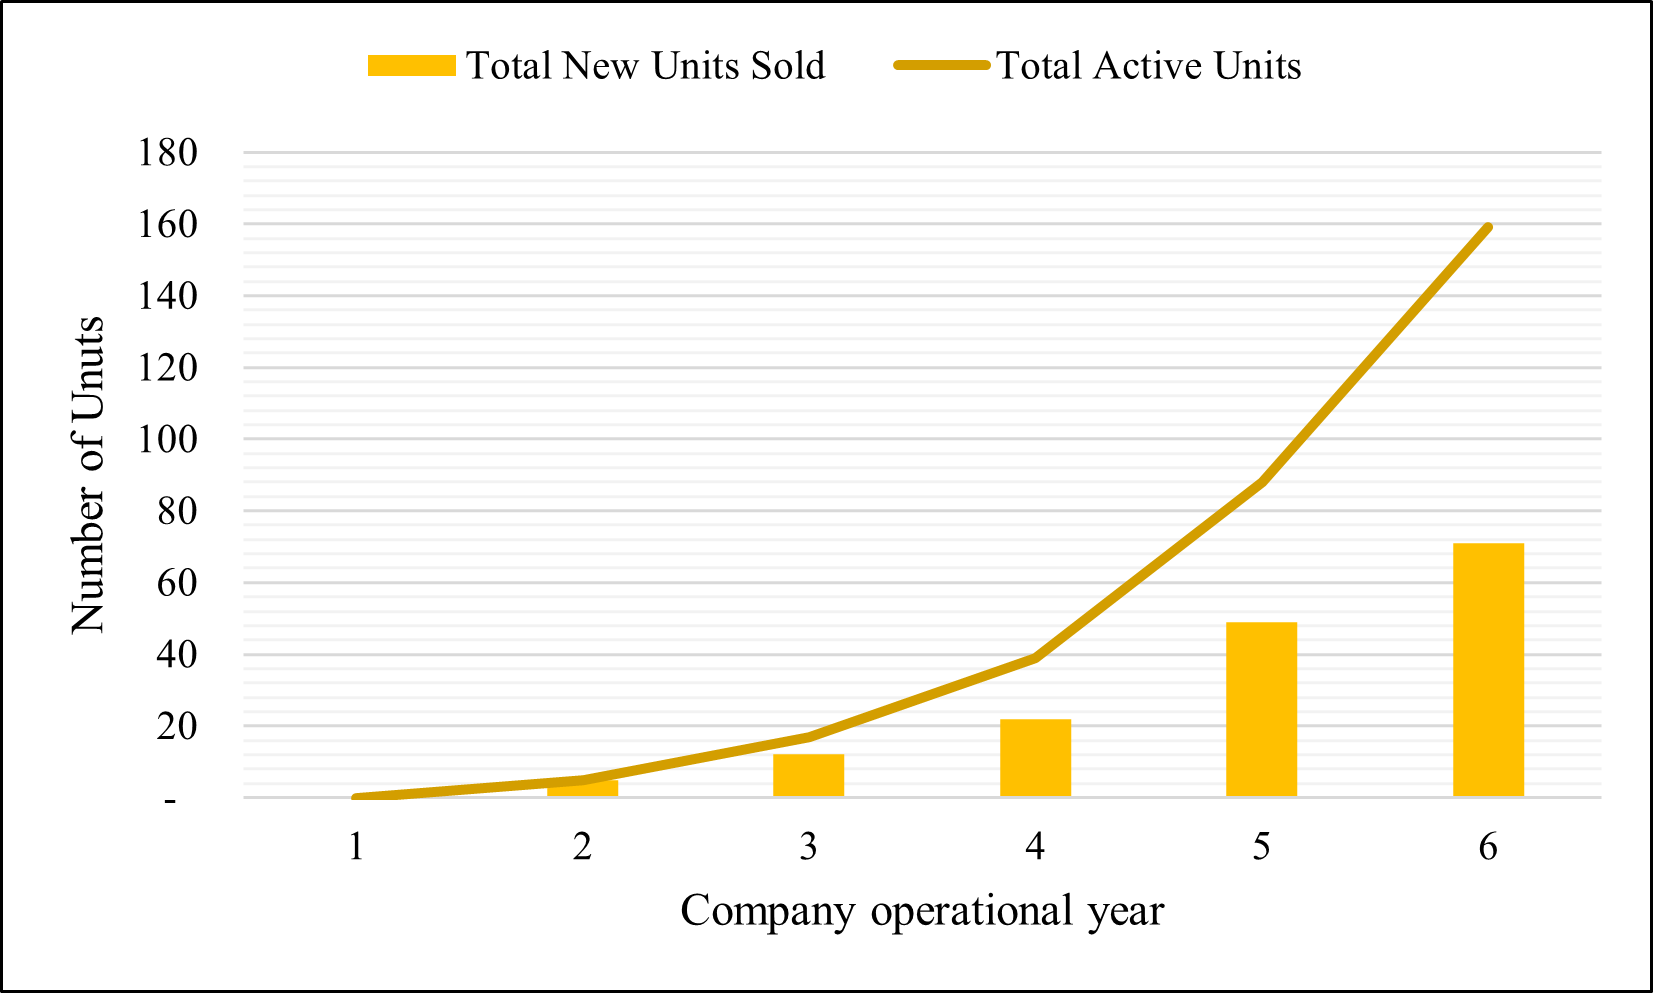
\includegraphics{figures/Chart Number of Units.png}
 %   \caption{Projected BELLONA sales ramp and active installed base from Year 1 to Year 6.}
 %   \label{fig:roi_sales_ramp}
%\end{figure}

\section{Revenue, Cost, and Profitability}

Revenue is split into one-time hardware sales and recurring annual maintenance/service income. The one-time sales price is EUR 24,875 per complete deployable UAS package, while each active unit generates EUR 11,999 in annual maintenance and service revenue. This recurring revenue covers inspection, maintenance support, software and device management, replacement parts, and continued operational readiness. By Year 6, annual maintenance and service revenue slightly exceeds new-unit hardware revenue, meaning the company becomes partly supported by the installed base rather than only by continuous new sales.

%\begin{figure}[H]
   %\centering
    %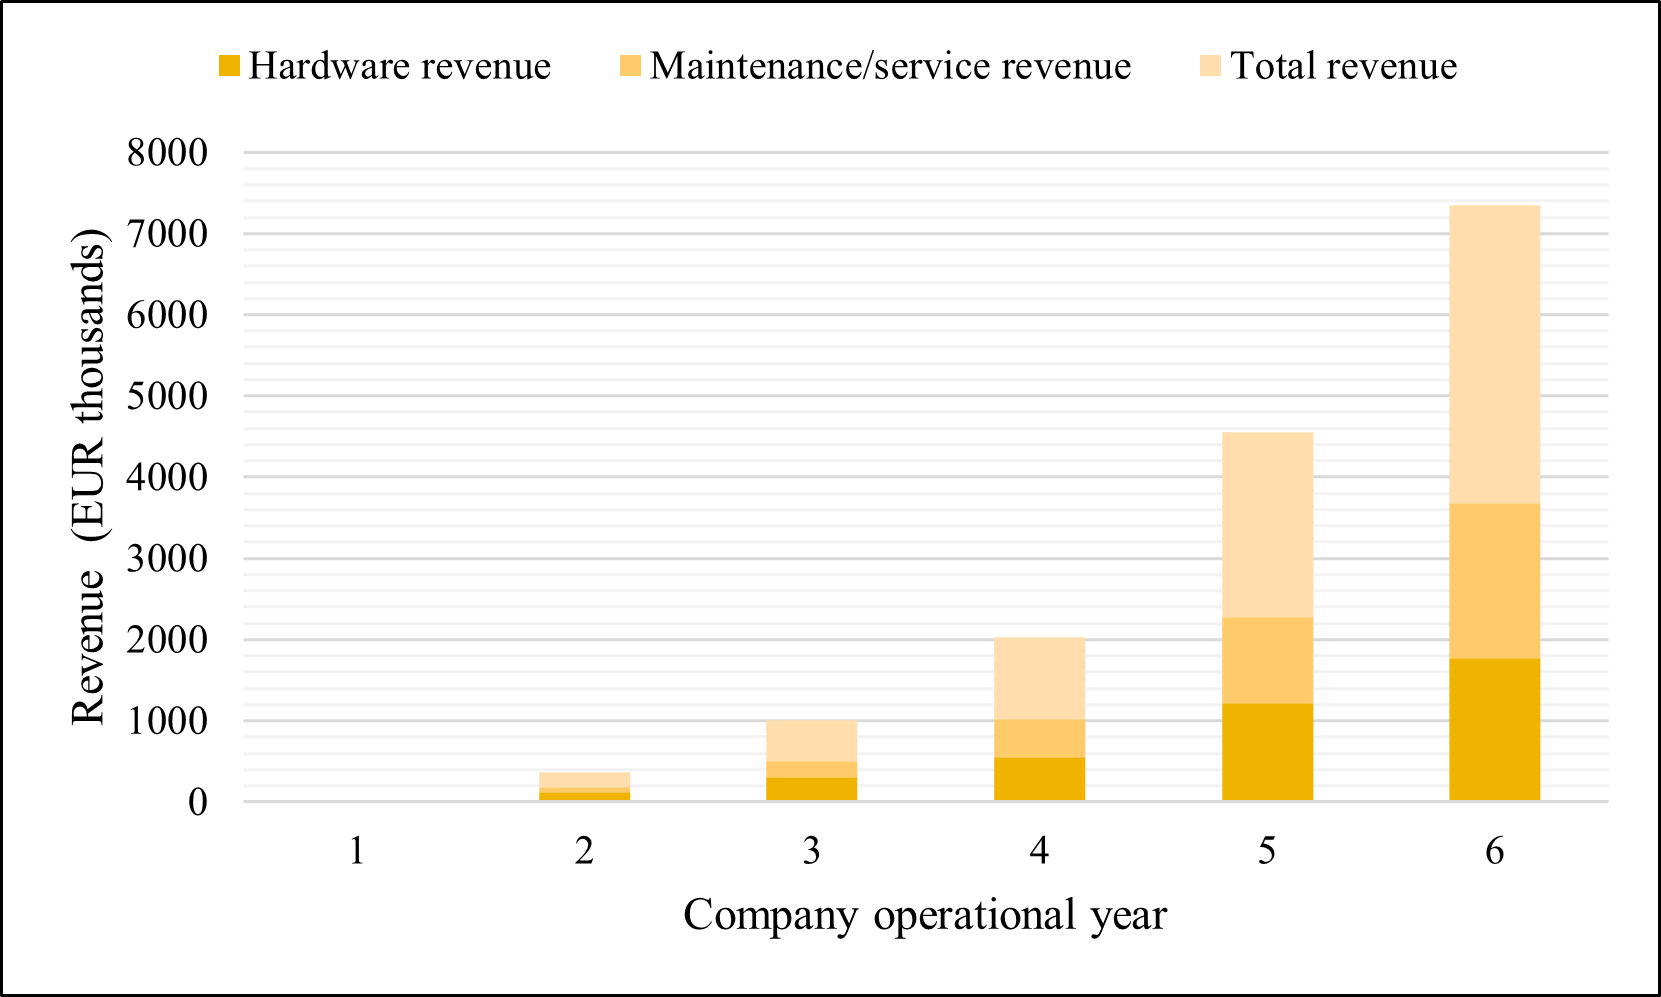
\includegraphics{figures/Chart revenue.png}
   % \caption{Revenue split between new-unit sales and recurring annual maintenance/service revenue.}
   % \label{fig:roi_revenue_split}
%\end{figure}

The production cost model separates one-time COGS from recurring COGS. One-time COGS are incurred when a new BELLONA unit is produced and delivered, including the airframe, propulsion system, power system, sensors, flight controller, net and launcher system, manufacturing, installation, and integration items. Recurring COGS are linked to the active installed base and include routine maintenance parts, cloud and device management, quality-assurance allowance, and technician support.

At unit level, the hardware gross margin is moderate but positive. A new unit is sold for EUR 24,875 and has one-time COGS of EUR 17,100, giving a gross margin of approximately 31\%. The annual service margin is higher: each active unit generates EUR 11,999 in maintenance/service revenue per year, while recurring COGS are EUR 2,400 per active unit per year. This gives an annual service gross margin of approximately 80\%, showing why the installed base is financially important.

%\begin{figure}[H]
  %  \centering
  %  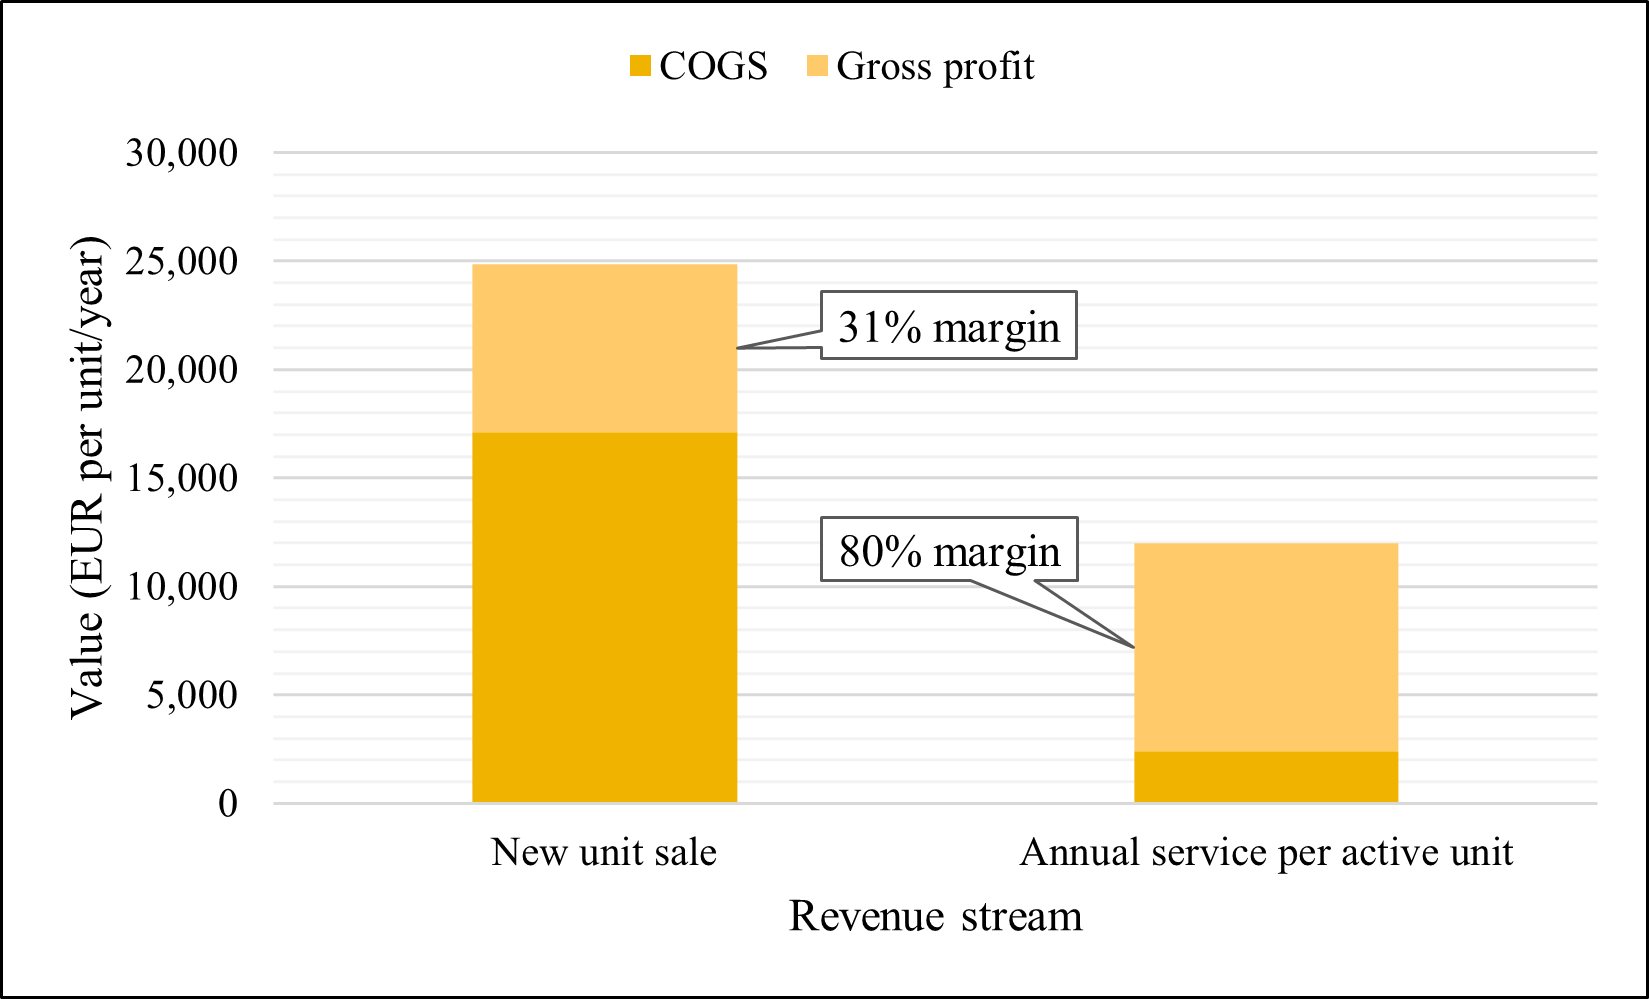
\includegraphics{figures/Chart Profits.png}
  %  \caption{Unit-level gross margins for hardware sales and annual maintenance/service revenue.}
  %  \label{fig:roi_unit_economics}
%\end{figure}

The direct operational cost is considered separately from the company profit-and-loss statement. The current estimate is EUR 150 per mission, covering operator-side energy use, mission preparation, reset or consumables, inspection, and minor wear.  In the first years, the company remains loss-making because the installed base is still small while development and market-entry costs are already incurred. By Year 6, BELLONA reaches operational profitability, with EUR 3.67M in revenue, approximately EUR 2.08M in gross profit, and EUR 89k in net profit after operating expenses and tax.

%\begin{figure}[H]
  %  \centering
  %  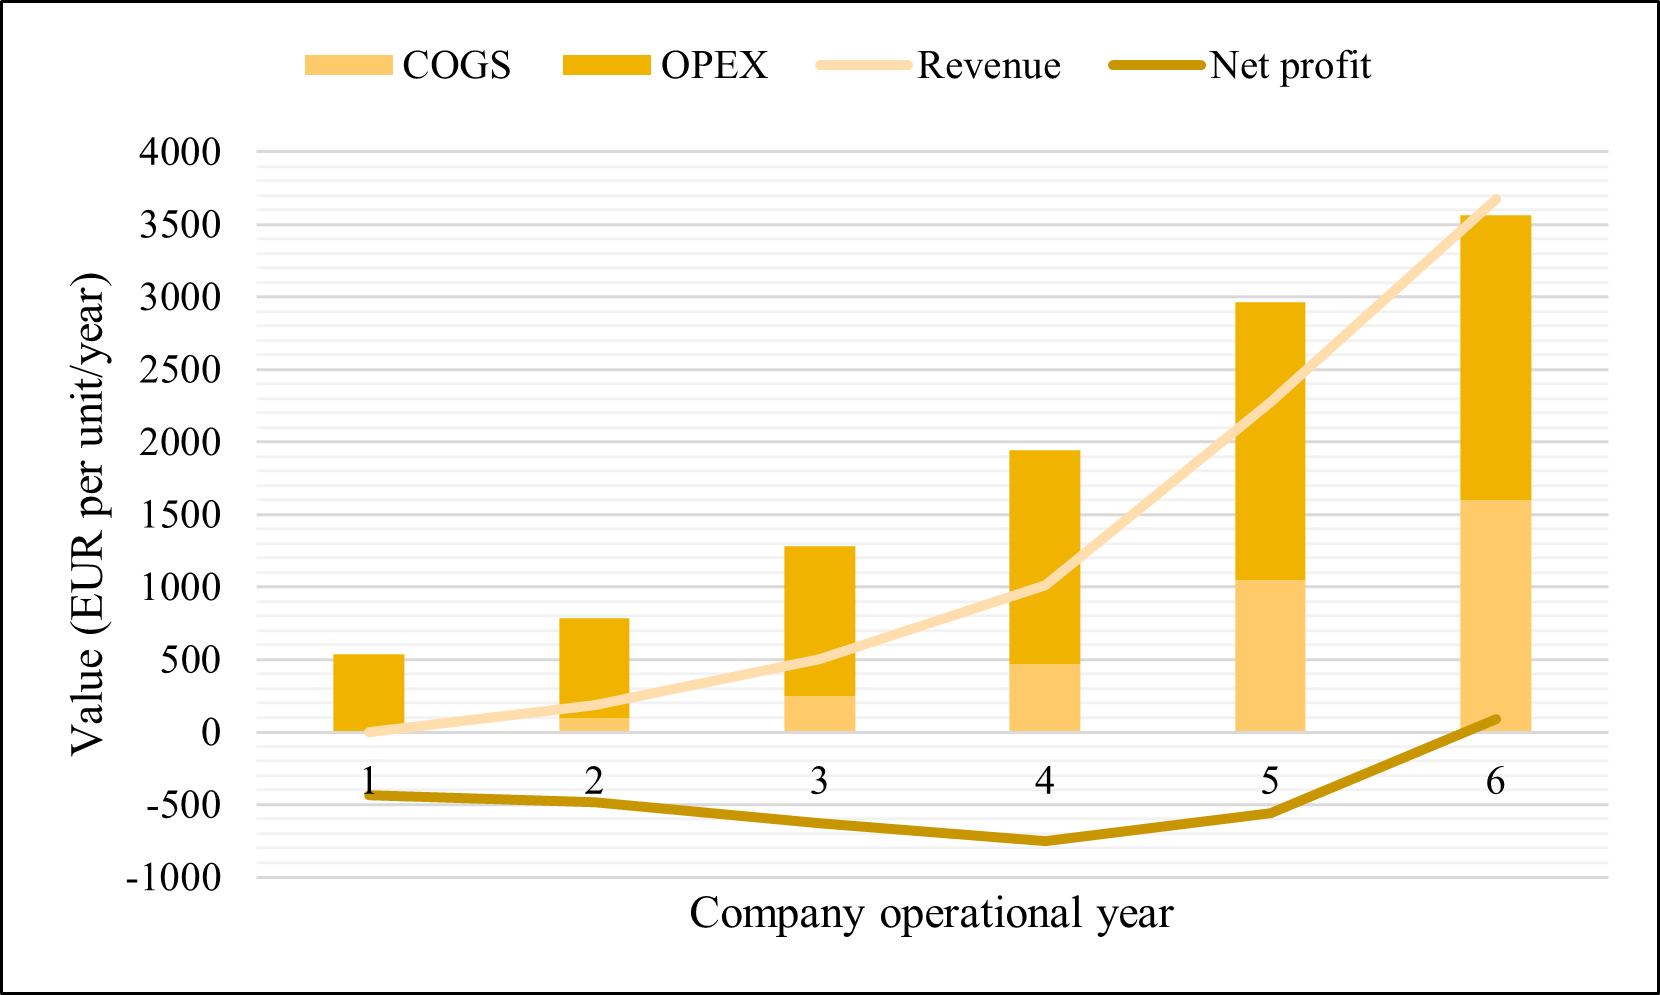
\includegraphics{figures/Chart P&L.png}
  %  \caption{Profit-and-loss development from Year 1 to Year 6.}
  %  \label{fig:roi_pl_development}
%\end{figure}

\section{Timeline and Funding Plan}

The financial timeline follows the transition from development to commercial scale-up. Year 1 covers prototype and Minimum Viable Product (MVP) validation, while commercial entry starts in Year 2 with the first unit sales. Years 3 to 5 represent scale-up, where the installed base grows but operating cash flow remains negative because the company must still fund R\&D, testing, certification preparation, staffing, field support, and sales activity. Year 6 is selected as the target year because it is the first year with positive net profit and positive operating cash flow.

This timeline is consistent with the selected architecture. Concept A still requires development of the tail-sitter Vertical Take-Off and Landing (VTOL) platform, upward net-launching mechanism, tether and reel integration, sensor package, and recovery procedures before large-scale deployment. Therefore, development cost is captured through the full funding requirement needed to cover development, validation, staffing, operating losses, and investment activities before profitability is reached.

\begin{table}[H]
    \centering
    \caption{Financial timeline and funding plan. Values are rounded and expressed in EUR thousands.}
    \label{tab:roi_funding_plan}
    \renewcommand{\arraystretch}{1}
    \setlength{\tabcolsep}{5pt}
    \small
    \begin{tabular}{
        c
        @{\hspace{0.35cm}} p{0.25\textwidth}
        @{\hspace{0.25cm}} r
        @{\hspace{0.25cm}} r
        @{\hspace{0.25cm}} r
        @{\hspace{0.25cm}} r
        @{\hspace{0.25cm}} r
        @{\hspace{0.25cm}} r
    }
        \toprule
        \textbf{Year} 
        & \textbf{Main phase} 
        & \makecell{\textbf{New}\\\textbf{units}} 
        & \makecell{\textbf{Active}\\\textbf{units}} 
        & \makecell{\textbf{Operating}\\\textbf{cash flow}} 
        & \makecell{\textbf{Investing}\\\textbf{cash flow}} 
        & \textbf{Financing} 
        & \makecell{\textbf{Closing}\\\textbf{cash}} \\
        \midrule
        1 & Prototype, MVP, pilot validation        & 0  & 0   & -420 & -70 & 1,050 & 560 \\
        2 & First commercial contracts              & 5  & 5   & -463 & -25 & 200   & 271 \\
        3 & Early customer expansion                & 12 & 17  & -598 & -40 & 400   & 33  \\
        4 & Scale-up and team expansion             & 22 & 39  & -710 & -55 & 1,500 & 769 \\
        5 & Larger deployment ramp                  & 49 & 88  & -518 & -70 & 0     & 181 \\
        6 & Target year / operational profitability & 71 & 159 & 131  & -40 & 0     & 272 \\
        \bottomrule
    \end{tabular}
\end{table}

The funding plan is staged to match the company cash-flow requirement. A first equity round of EUR 1.0M and EUR 50k in grant funding are assumed in Year 1. Additional grant funding of EUR 200k and EUR 400k is included in Years 2 and 3, followed by a larger EUR 1.5M equity round in Year 4 to support sales, staffing, field support, and production scale-up.

Total external financing required before the target year is EUR 3.15M. This is the practical funding requirement needed to bring BELLONA from development to operational profitability. The lowest projected cash balance occurs in Year 3, at approximately EUR 33k, after which the Year 4 equity round restores sufficient liquidity for scale-up. In Year 6, the company reaches positive operating cash flow of EUR 131k and closing cash of EUR 272k.

\todo{add FUNDING FIGURE WHICH JAN REMOVED}

\section{ROI Interpretation}

The Design Synthesis Exercise (DSE) definition of ROI is used for the target-year calculation. In Year 6, BELLONA reaches EUR 3.674M in revenue and EUR 89.25k in net profit after tax. Interpreting total cost as revenue minus net profit gives:

\begin{equation}
    ROI_{Y6} =
    \frac{89.25}{3673.97 - 89.25}
    = 0.0249 \approx 2.5\%
    \label{eq:roi_y6}
\end{equation}

The target-year ROI is therefore positive but modest. This is expected because Year 6 is the first year of operational profitability, not a mature steady-state year. The cumulative return over Years 1--6 remains negative because the company must first absorb development, testing, certification preparation, staffing, and market-entry losses.

Overall, the updated financial model shows that BELLONA has a credible path to operational profitability. The business is not justified by hardware sales alone; its viability depends on combining new-unit sales with high-margin annual maintenance and service revenue from the growing installed base. By Year 6, the model reaches 159 active units, EUR 3.67M in annual revenue, positive net profit, positive operating cash flow, and a positive target-year ROI of 2.5\%. However, full investment payback requires continued growth beyond Year 6.

